\section{Entwurf}

\label{sec_impl_architecture}

Architektur








\subsection*{Ansätze zum Eingriff in den OSSIM-Datenfluss(?)}

\todo{Hier oder in Entwurf?}

Für den Eingriff zur Pseudonymisierung der Logdaten bieten sich verschiedene Stellen im Datenfluss von OSSIM an. In diesem Abschnitt sollen die verschiedenen Möglichkeiten dargestellt und gegeneinander abgewogen werden. Eine Übersicht über die verschiedenen Stellen bietet Abbildung \ref{fig:ossim_data_access_point}.

\begin{figure}[]
    \centering
        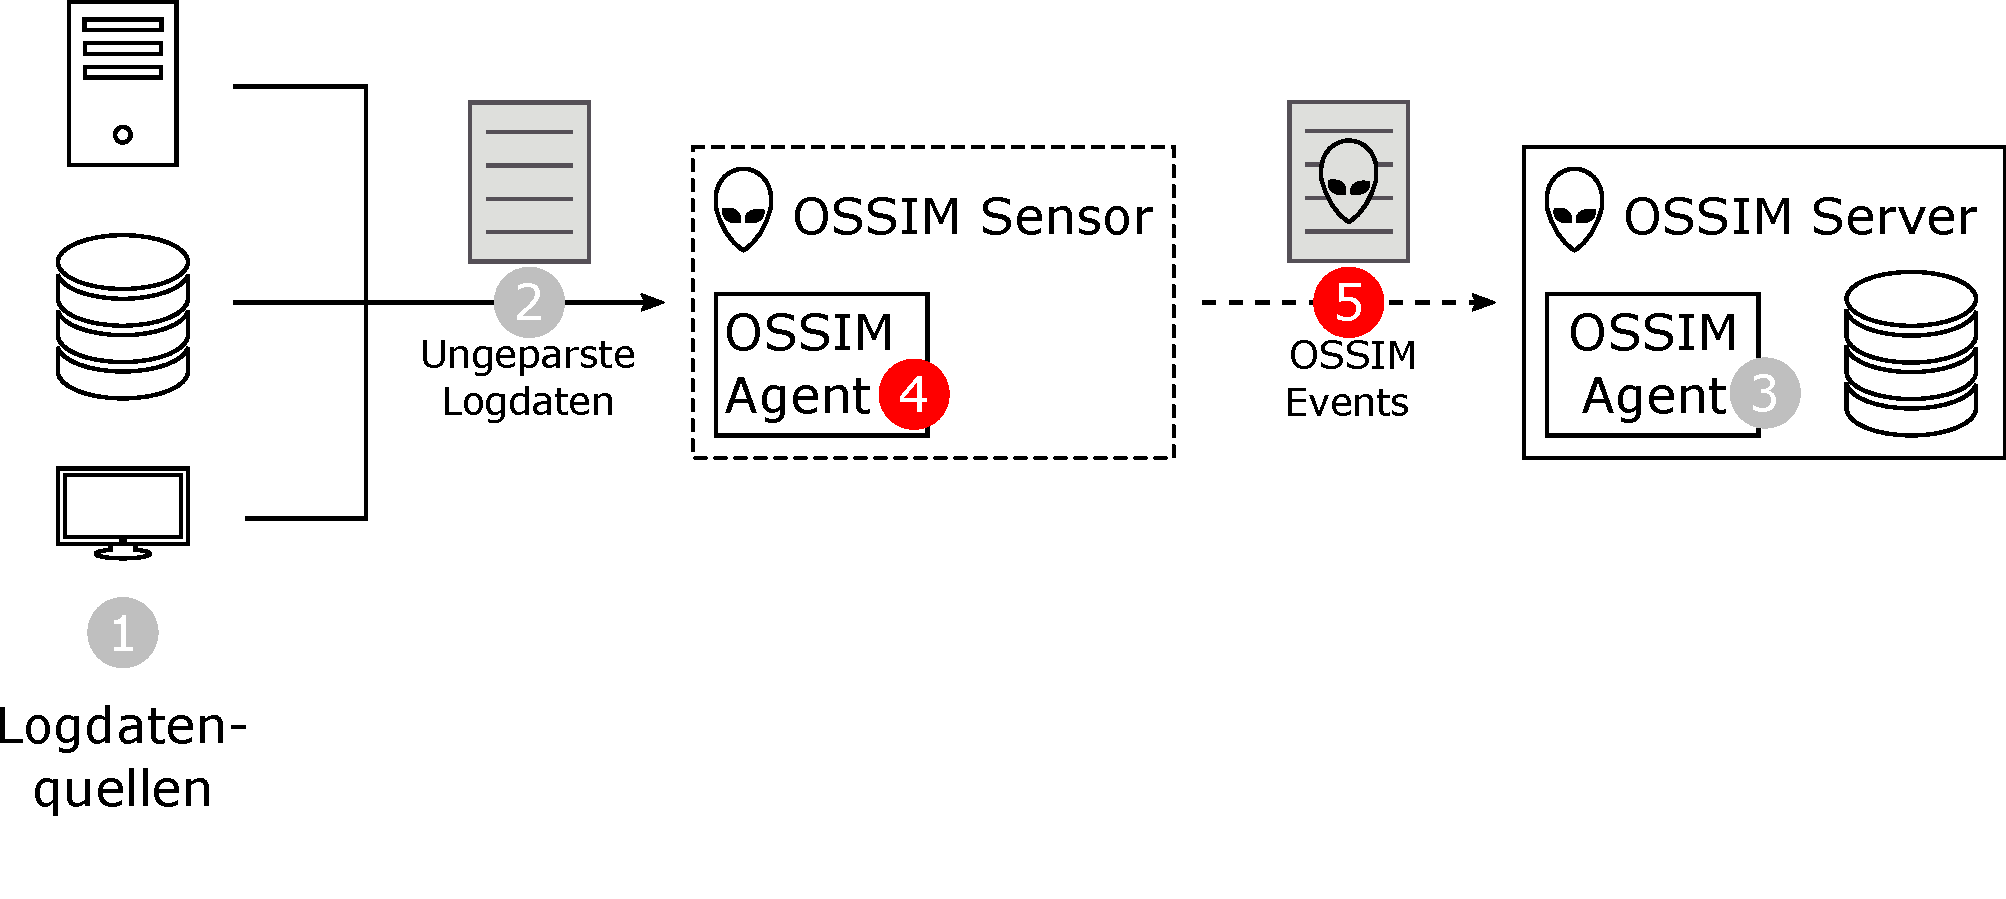
\includegraphics[width=0.9\textwidth]{dia/ossim_data_access_point.pdf}
    \caption{Möglichen Eingriffspunkte in den OSSIM-Datenfluss.}
    \label{fig:ossim_data_access_point}
\end{figure}

\begin{enumerate}

\item \textbf{In der Quelle der Logdaten}\\
  Bei diesem Ansatz werden die Daten bereits pseudonymisiert, bevor sie die Datenquelle verlassen. Auch wenn dieser Ansatz aus datenschutztechnischer Sicht die beste Möglichkeit darstellen würde, so ist er doch nicht umsetzbar, da hierzu jede mögliche Quelle von Logdaten universell verändert werden müsste.

\item \textbf{Syslog-Proxy}\\
  Dieser Ansatz pseudonymisiert die Daten vor dem ersten Kontakt mit einer OSSIM-Komponente, indem Datenquellen ihre Logdaten an einen Proxy senden, der die Daten pseudonymisiert und erst anschließend an OSSIM weiterreicht. Hierdurch wird erreicht, dass die Daten zu keiner Zeit nicht-pseudonymisiert in OSSIM vorliegen. Ein Nachteil dieser Lösung ist, dass sie das Parsen und Neuzusammensetzen der Logdaten im Proxy erfordert. \todo{Beschreibung erweitern - analog zu Plugins in OSSIM}

\item \textbf{Patchen des OSSIM-Sensor-Agents}\\
  Bei dieser Lösung müsste der OSSIM-Agent des Sensors so verändert werden, dass vor dem Senden der Events an den Server die Pseudonymisierung stattfindet. Daten erreichen den OSSIM-Server nur pseudonymisiert und mehrfaches Parsen wie in der zweiten Lösung wird verhindert. Auf der anderen Seite erfordert diese Lösung einen Eingriff in die Funktionsweise von OSSIM, was beispielsweise bei Updates von OSSIM zu Problemen führen kann. Außerdem liegen die Daten zu Beginn in nicht-pseudonymisierter Form im Sensor vor. \todo{Syslog-Problematik erwähnen} Zusätzlich erfordert diese Lösung die verteilte Installation von OSSIM-Sensor und -Server, schließt also die All-In-One-Installation aus.
  
\item \textbf{Sensor-Server-Proxy}\\
  Hier wird ein Proxy zwischen Sensor und Server geschaltet, der bereits geparste Events pseudonymisiert und anschließend an den Server sendet. Dieser Ansatz würde mehrfaches Parsen verhindern und dafür sorgen, dass nur pseudonymisierte Logdaten den OSSIM-Server erreichen. Wie die vorhergehende Lösung würde er jedoch nur in der verteilten Installation funktionieren und zusätzlich in die Kommunikation zwischen Sensor und Server aktiv eingreifen, was im Hinblick auf die Nachrichtenintegrität\footnote{
    In der aktuellen Version von OSSIM werden Nachrichten unverschlüsselt und nicht signiert zwischen Sensor und Server versendet, aber zu hoffen ist, dass dieser Zustand sich in zukünftigen Versionen noch ändert.
  } und auch auf geändertes Verhalten nach Updates von OSSIM einen Nachteil darstellt.
  
\item \textbf{Patchen des OSSIM-Servers}\\
  Die letzte Möglichkeit ist das Verändern des OSSIM-Servers selbst. Diese Lösung ist vergleichbar mit der dritten Möglichkeit. Zusätzlich würde sie bei der verteilten sowie bei der All-In-One-Installation funktionieren, auf der anderen Seite aber zulassen, dass nicht-pseudonymisierte Events sogar noch direkt auf dem Server vorliegen.

\end{enumerate}

Insbesondere der aus dentenschutztechnischer Sicht relevante Vorteil, dass die Daten bereits pseudonymisiert in allen OSSIM-Komponenten eintreffen, ließ die Entscheidung auf die zweite Möglichkeit fallen. Dass die Lösung außerdem noch für beide Varianten der OSSIM-Installation möglich ist und keine Anpassungen an OSSIM selbst benötigt, wiegt den Nachteil des zusätzlichen Parsens und wieder Zusammensetzens der Lognachricht bei Weitem auf.\todo{Auch auf Angreifermodell beziehen}